% !TeX root = ../presentation.tex

\section{Data Spaces}

\begin{frame}{Inter-Organisational Information Systems (IOIS) \footnotesize\cite{mollerIndustrialDataEcosystems2024}}
    \begin{columns}
        \begin{column}{0.6\textwidth}
            \begin{itemize}
                \item \alert{bilaterale} Beziehungen, bspw. Lieferketten
                \item tiefe Integration, automatisiertes Data Sharing
                \item zweckgebunden, bspw. Koordinierung und Optimierung von Lieferketten
                
                \note{
                    \begin{itemize}
                        \item Mittel zum Zweck
                    \end{itemize}
                }
                
                \item<2-> mangelndes Vertrauen, streng formalisierte Nutzungsrichtlinien
                \item<2-> keine Daten teilen? $\to$ Ineffizienz $\to$ Verlust
                \item<2-> Herausforderungen bei Skalierung % Datenaustausch, Kontrolle
            \end{itemize}
        \end{column}
        
        \begin{column}{0.4\textwidth}
            \begin{figure}
                
\includegraphics[height=0.5\textheight]{./assets/iois_architecture.drawio.pdf}
                \caption{IOIS Architektur}
            \end{figure}
        \end{column}
    \end{columns}
\end{frame}


\begin{frame}{Data Intermediaries \footnotesize\cite{mollerIndustrialDataEcosystems2024}}
    \begin{columns}
        \begin{column}{0.6\textwidth}
            \begin{itemize}
                \item Gleichgewicht zwischen erhaltenem und gegebenem Aufwand
                \item Daten als strategische Ressource
                
                \note{
                    \begin{itemize}
                        \item dynamisch, geteilter Zweck statt Mittel zum Zweck
                        \item ermöglichen neue Geschäfte und Optimierung von Prozessen
                    \end{itemize}
                }
                
                \item<2-> Interaktion und Kooperation \alert{multilateraler} Akteure
                \item<2-> Data User, Data Provider, Data Intermediary
                
                \item<3-> offener, dynamischer Datenaustausch
                \item<3-> Netzwerkeffekte, Förderung von Innovation
            \end{itemize}
        \end{column}
        
        \begin{column}{0.4\textwidth}
            \begin{figure}
                \centering
                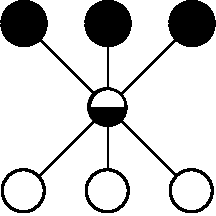
\includegraphics[height=0.5\textheight]{./assets/industrial_de_architecture.drawio.pdf}
                \caption{Data Intermediary}
            \end{figure}
        \end{column}
    \end{columns}
\end{frame}


\begin{frame}{Data Spaces \footnotesize\cite{mollerIndustrialDataEcosystems2024}}
    \begin{columns}
        \begin{column}{0.6\textwidth}
            \begin{itemize}
                \item Vereinen von IOIS und Data Intermediaries
                \item dezentrale Speicherung von Daten bei Provider
                
                \item<0|handout:0> Datenintegration auf semantische Ebene
                \begin{itemize}
                    \item[$\to$]<0|handout:0> kein einheitliches Daten"=Schema notwendig
                \end{itemize}
                \item<0|handout:0> bilateraler Datenaustausch
                \item<0|handout:0> Vermittlung zwischen Data User und Provider
                \item<0|handout:0> technische Garantie von Datensouveränität
                \item<0|handout:0> geteilter Raum für vertrauenswürdiges Data Sharing $\to$ Optimierung, Innovation
            \end{itemize}
        \end{column}
        
        \begin{column}{0.4\textwidth}
            \begin{figure}
                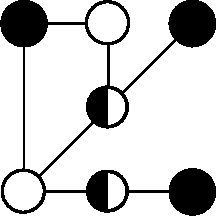
\includegraphics[height=0.5\textheight]{./assets/data_space_architecture.drawio.pdf}
                \caption{Data Space Architektur}
            \end{figure}
        \end{column}
    \end{columns}
\end{frame}


\begin{frame}[c]{Einschub: Zentrale vs. Dezentrale Datenspeicherung}
    \vspace{1.5em}

    \begin{figure}
        \centering
        \begin{subfigure}{0.4\textwidth}
            \centering
            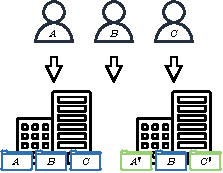
\includegraphics[height=5cm]{./assets/central.drawio.pdf}
        \end{subfigure}
        %
        \hspace{2cm}
        %
        \only<2->{
            \begin{subfigure}{0.4\textwidth}
                \centering
                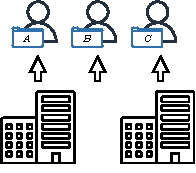
\includegraphics[height=5cm]{./assets/decentral.drawio.pdf}
            \end{subfigure}
        }
        %
        \caption{zentralisierte vs. dezentralisierte Datenspeicherung}
    \end{figure}

    \note{
        \begin{itemize}
            \item kurzer Einschub: was heißt dezentrale Speicherung?
        \end{itemize}

        \textbf{Zentral}
        \begin{itemize}
            \item von vorhin bekannt
            \item rechts dasselbe in grün, jedoch eben nicht, sondern veraltet
            \item Duplikat $\to$ Inkonsistenz
        \end{itemize}

        \textbf{Dezentral}
        \begin{itemize}
            \item Daten bei Nutzenden / Data Provider $\to$ Konsistenz
            \item Kontrolle über Zugang, nur wenn notwendig
        \end{itemize}
    }
\end{frame}


\begin{frame}{Data Spaces \footnotesize\cite{mollerIndustrialDataEcosystems2024}}
    \begin{columns}
        \begin{column}{0.6\textwidth}
            \begin{itemize}
                \item Vereinen von IOIS und Data Intermediaries
                \item dezentrale Speicherung von Daten bei Provider
                
                \item<2-> Datenintegration auf semantische Ebene
                \begin{itemize}
                    \item[$\to$]<2-> kein einheitliches Daten"=Schema notwendig
                \end{itemize}
                
                \item<3-> bilateraler Datenaustausch
                \item<3-> Vermittlung zwischen Data User und Provider
                
                \note{
                    \begin{itemize}
                        \item bilat. Datenaust.: vgl. IOIS
                        \item Vermittlung DU / DP: vgl. Data Intermediary // vgl. Adapter / Mediator
                        \item prinzipiell überhaupt eine Chance, dass ich an benötigte Daten komme\\
                            $\to$ Daten-Lieferketten, muss zu best. Domäne kommen
                    \end{itemize}
                }

                \item<4-> technische Garantie von Datensouveränität
                \item<4-> geteilter Raum für vertrauenswürdiges Data Sharing $\to$ Optimierung, Innovation

                \note{
                    \textbf{technische Garantie von Datensouveränität}
                    \begin{itemize}
                        \item[$\to$] Überwindung betriebl. Barrieren // Kontrolle über Zugriff und Verwendung bei Provider
                    \end{itemize}

                    \textbf{geteilter Raum für vertr. DSh}
                    \begin{itemize}
                        \item flexible betriebliche Strukturen
                        \item Zugang nur für bestimmte Akteure $\to$ \emph{Trusted Pool}
                        \item sicheres, vertrauenswürdiges Data Sharing
                    \end{itemize}
                }
            \end{itemize}
        \end{column}
        
        \begin{column}{0.4\textwidth}
            \begin{figure}
                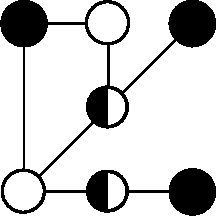
\includegraphics[height=0.5\textheight]{./assets/data_space_architecture.drawio.pdf}
                \caption{Data Space Architektur}
            \end{figure}
        \end{column}
    \end{columns}
\end{frame}


\begin{frame}{Data Ecosystems \footnotesize\cite{mollerIndustrialDataEcosystems2024}}
    \begin{columns}
        \begin{column}{0.6\textwidth}
            \begin{itemize}
                \item Kapselung $\to$ Data Space als Data Provider
                \note{
                    \scriptsize
                    \begin{itemize}
                        \item merkt man nicht, wenn DS größer wird
                    \end{itemize}
                }
                
                \item[$\Rightarrow$] \emph{globaler} Data Space?
                \begin{itemize}
                    \item<2-> Domänen-spezifisch, starke Kopplungen
                \end{itemize}

                \note{
                    \scriptsize
                    \hrule
                    \begin{itemize}
                        \item Datenstrukturen für spez. genau für diesen Teilbereich, aber trotzdem verknüpft\\
                            jede Domäne hat noch weitere Daten, interessiert andere Seite nicht
                    \end{itemize}
                }

                \item<3-> eigene Data Spaces für Domäne
                \item<3-> über Data Space hinweg: lose Kopplung
                
                \note{
                    \scriptsize
                    \hrule
                    \begin{itemize}
                        \item daher DS: erfüllen genau diesen gemeinsamen Zweck\\
                            bspw. komplette Medizindaten beim Arzt vs. nur relevante Daten für Studie
                    \end{itemize}
                }

                \item[$\Rightarrow$]<4-> Verschachtelung / Überlappung von Data Spaces
                \item[$\Rightarrow$]<4-> \alert{\emph{Data Ecosystem}}
                
                \note{
                    \scriptsize
                    \hrule
                    \begin{itemize}
                        \item DE: technische Integration über Schnittstellen\\
                            Datensouveränität \& Verhinderung großer Daten-Silos: verschachtelt $\land$ überlappend\\
                            Bild: DPr. oder DS $\to$ Kapselung
                        % \begin{itemize}
                        %     \item orange: Verbindung DS // oben rechts: nicht DS, trotzdem Zugriff
                        % \end{itemize}
                    \end{itemize}
                }

                    % Bild: Punkte können Data Prov. oder DS sein --> Kapselung, Verschachtelung
                    % orangene Linien: Verbindung von Data Spaces, lose Kopplung
                    % oben rechts: kein Teilnehmer aus DS von unten, aber trotzdem Zugriff auf rel. Daten
                
                % prinzipiell überhaupt eine Chance, dass ich an benötigte Daten komme
                % --> Daten-Lieferketten, muss zu best. Domäne kommen
                % brauche Kontrollen --> DS Connectors
                \item<5-> Integration über \emph{Data Space Connector}
                % vgl. Adapter (nur Weitergabe) oder Mediator (inkl. Kontrollmechanismen)
                % Kontrolle notwendig --> DS Connectors
                % bspw. Weitergabe von med. Daten an Forschungsinstitut
                %   muss anonymisiert erfolgen, nur best. Daten dürfen weitergegeben werden
                \item<5-> Governance"=Maßnahmen je Abstraktionsebene
                % Erfüllung rechtlicher Rahmenbedingungen
                % Ebene von DE, DS, Pod oder Ressourcen
                \item<5-> Erreichen gemeinsamer Ziele
                
                \note{
                    \scriptsize
                    \hrule
                    \begin{itemize}
                        \item überhaupt an Daten kommen $\to$ Daten-Lieferk., Kontrolle (med. Daten) $\to$ DS Connector // med. Daten\\
                            Gov.-Maßn.: Kontrollen, rechtl. Bed., Ebene von DE, DS, Pod oder Ress.
                    \end{itemize}
                }
            \end{itemize}
        \end{column}

        \begin{column}{0.4\textwidth}
            \only<4->{
                \begin{figure}
                    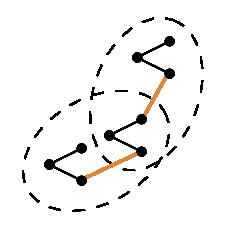
\includegraphics[height=5cm]{./assets/data_ecosystem_architecture.drawio.pdf}
                    \vspace{-1em}
                    \caption{Data Ecosystem}
                \end{figure}
            }
        \end{column}
    \end{columns}

    \note{
        \scriptsize
        \hrule
        \begin{itemize}
            \item Data Spaces erfüllen am meisten Kriterien, Wie kann das fkt? $\to$ Solid
        \end{itemize}
    }
\end{frame}
